%!TEX TS-program = xelatex

% biber 
% biblatex

\documentclass[12pt,a4paper, oneside]{extreport}

%%%%%%%%%% Математика %%%%%%%%%%
\usepackage{amsmath,amsfonts,amssymb,amsthm,mathtools}
% Показывать номера только у тех формул, на которые есть \eqref{} в тексте.
%\mathtoolsset{showonlyrefs=true}
%\usepackage{leqno} % Нумерация формул слева
%\usepackage{tipa} %Для формулки из логитов


% \noindent
% уравнение ()

\usepackage{hyphenat}


%%%%%%%%%% Шрифты %%%%%%%%
\usepackage[english, russian]{babel} % выбор языка для документа
\usepackage[utf8]{inputenc} % задание utf8 кодировки исходного tex файла
\usepackage[X2,T2A]{fontenc}        % кодировка

\usepackage{fontspec}         % пакет для подгрузки шрифтов
\setmainfont{Times New Roman}       % задаёт основной шрифт документа

\usepackage{unicode-math}      % пакет для установки математического шрифта
\setmathfont{Asana-Math.otf}    % шрифт для математики

% Конкретный символ из конкретного шрифта
% \setmathfont[range=\int]{Neo Euler}




%%%%%%%%%% Работа с картинками %%%%%%%%%
\usepackage{graphicx}                  % Для вставки рисунков
\usepackage{graphics}
\graphicspath{{images/}{pictures/}}    % можно указать папки с картинками
\usepackage{wrapfig}                   % Обтекание рисунков и таблиц текстом


%%%%%%%%%% Работа с таблицами %%%%%%%%%%
\usepackage{tabularx}            % новые типы колонок
\usepackage{tabulary}            % и ещё новые типы колонок
\usepackage{array,delarray}      % Дополнительная работа с таблицами
\usepackage{longtable}           % Длинные таблицы
\usepackage{multirow}            % Слияние строк в таблице
\usepackage{float}               % возможность позиционировать объекты в нужном месте

\usepackage{booktabs}            % таблицы как в книгах
% Заповеди из документации к booktabs:
% 1. Будь проще! Глазам должно быть комфортно
% 2. Не используйте вертикальные линни
% 3. Не используйте двойные линии. Как правило, достаточно трёх горизонтальных линий
% 4. Единицы измерения - в шапку таблицы
% 5. Не сокращайте .1 вместо 0.1
% 6. Повторяющееся значение повторяйте, а не говорите "то же"
% 7. Есть сомнения? Выравнивай по левому краю!

%  вычисляемые колонки по tabularx
\newcolumntype{C}{>{\centering\arraybackslash}X}
\newcolumntype{L}{>{\raggedright\arraybackslash}X}
\newcolumntype{Y}{>{\arraybackslash}X}
\newcolumntype{Z}{>{\centering\arraybackslash}X}


%%%%%%%%%% Графика и рисование %%%%%%%%%%
\usepackage{tikz, pgfplots}      % язык для рисования графики из latex'a

%%%%%%%%%% Гиперссылки %%%%%%%%%%
\usepackage{xcolor}              % разные цвета

\usepackage{hyperref}
\hypersetup{
	unicode=true,           % позволяет использовать юникодные символы
	colorlinks=true,       	% true - цветные ссылки, false - ссылки в рамках
	urlcolor =blue,         % цвет ссылки на url
	linkcolor=black,        % внутренние ссылки
	citecolor=black,        % на библиографию
	breaklinks              % если ссылка не умещается в одну строку, разбивать ли ее на две части?
}


%%%%%%%%%% Другие приятные пакеты %%%%%%%%%
\usepackage{multicol}       % несколько колонок
\usepackage{verbatim}       % для многострочных комментариев
\usepackage{cmap} % для кодировки шрифтов в pdf

\usepackage{enumitem} % дополнительные плюшки для списков
%  например \begin{enumerate}[resume] позволяет продолжить нумерацию в новом списке

\usepackage{todonotes} % для вставки в документ заметок о том, что  осталось сделать
% \todo{Здесь надо коэффициенты исправить}
% \missingfigure{Здесь будет Последний день Помпеи}
% \listoftodos --- печатает все поставленные \todo'шки




\usepackage[bottom]{footmisc}

%%%%%%%%%%%%%% ГОСТОВСКИЕ ПРИБАМБАСЫ %%%%%%%%%%%%%%%

%%% размер листа бумаги
\usepackage[paper=a4paper,top=15mm, bottom=15mm,left=35mm,right=10mm,includehead]{geometry}


\usepackage{setspace}
\setstretch{1.33}     % Межстрочный интервал
\setlength{\parindent}{1.25cm} % Красная строка.


%\flushbottom       % Эта команда заставляет LaTeX чуть растягивать строки, чтобы получить идеально прямоугольную страницу
\righthyphenmin=2  % Разрешение переноса двух и более символов
\widowpenalty=10000  % Наказание за вдовствующую строку (одна строка абзаца на этой странице, остальное --- на следующей)
%\clubpenalty=10000  % Наказание за сиротствующую строку (омерзительно висящая одинокая строка в начале страницы)
\tolerance=1000     % Ещё какое-то наказание.


% Нумерация страниц сверху по центру
\usepackage{fancyhdr}
\pagestyle{fancy}
\fancyhead{ } % clear all fields
\fancyfoot{ } % clear all fields
\fancyhead[C]{\thepage}
% Чтобы не прорисовывалась черта!
\renewcommand{\headrulewidth}{0pt}


% Нумерация страниц с надписью "Глава"
\usepackage{etoolbox}
\patchcmd{\chapter}{\thispagestyle{plain}}{\thispagestyle{fancy}}{}{}


%%% Заголовки
\usepackage[indentfirst]{titlesec}{\raggedleft}
% Заголовки по левому краю
% опция identfirst устанавливает отступ в первом абзаце



% В Linux этот пакет сделан косячно. Исправляет это следующий непонятный кусок кода.
\makeatletter
\patchcmd{\ttlh@hang}{\parindent\z@}{\parindent\z@\leavevmode}{}{}
\patchcmd{\ttlh@hang}{\noindent}{}{}{}
\makeatother


% Редактирования Глав и названий
\titleformat{\chapter}
{\normalfont\large\bfseries}
{\thechapter }{0.5 em}{}

% Редактирование ненумеруемых глав chapter* (Введение и тп)
\titleformat{name=\chapter,numberless}
{\centering\normalfont\bfseries\large}{}{0.25em}{}

% Убирает чеканутые отступы вверху страницы
\titlespacing{\chapter}{0pt}{-\baselineskip}{\baselineskip}

% Более низкие уровни
\titleformat{\section}{\bfseries}{\thesection}{0.5 em}{}
\titleformat{\subsection}{\bfseries}{\thesubsection}{0.5 em}{}

\titlespacing*{\section}{0 pt}{\baselineskip}{\baselineskip}
\titlespacing*{\subsection}{0 pt}{\baselineskip}{\baselineskip}


% Содержание. Команды ниже изменяют отступы и рисуют точечки!
\usepackage{titletoc}

\titlecontents{chapter}
[1em] %
{\normalsize}
{\contentslabel{1 em}}
{\hspace{-1 em}}
{\normalsize\titlerule*[10pt]{.}\contentspage}

\titlecontents{section}
[3 em] %
{\normalsize}
{\contentslabel{1.75 em}}
{\hspace{-1.75 em}}
{\normalsize\titlerule*[10pt]{.}\contentspage}

\titlecontents{subsection}
[6 em] %
{\normalsize}
{\contentslabel{3 em}}
{\hspace{-3 em}}
{\normalsize\titlerule*[10pt]{.}\contentspage}


% Правильные подписи под таблицей и рисунком
% Документация к пакету на русском языке!
\usepackage[tableposition=top, singlelinecheck=false]{caption}
\usepackage{subcaption}


\DeclareCaptionStyle{base}%
[justification=centering,indention=0pt]{}
\DeclareCaptionLabelFormat{gostfigure}{Рисунок #2}
\DeclareCaptionLabelFormat{gosttable}{Таблица #2}

\DeclareCaptionLabelSeparator{gost}{~---~}
\captionsetup{labelsep=gost}

\DeclareCaptionStyle{fig01}%
[margin=5mm,justification=centering]%
{margin={3em,3em}}
\captionsetup*[figure]{style=fig01,labelsep=gost,labelformat=gostfigure,format=hang}

\DeclareCaptionStyle{tab01}%
[margin=5mm,justification=centering]%
{margin={3em,3em}}
\captionsetup*[table]{style=tab01,labelsep=gost,labelformat=gosttable,format=hang}


% межстрочный отступ в таблице
\renewcommand{\arraystretch}{1.2}



% многостраничные таблицы под РОССИЙСКИЙ СТАНДАРТ
% ВНИМАНИЕ! Обязательно за CAPTION !
\usepackage{fr-longtable}



%Более гибкие спсики
\usepackage{enumitem}
% сообщаем окружению о том, что существует такая штук как нумерация русскими буквами.
\makeatletter
\AddEnumerateCounter{\asbuk}{\russian@alph}{щ}
\makeatother


%%% ГОСТОВСКИЕ СПИСКИ

% Первый тип списков. Большая буква.
\newlist{Enumerate}{enumerate}{1}

\setlist[Enumerate,1]{labelsep=0.5em,leftmargin=1.25em,labelwidth=1.25em,
	parsep=0em,itemsep=0em,topsep=0ex, before={\parskip=-1em},label=\arabic{Enumeratei}.}



% Второй тип списков. Маленькая буква.
\setlist[enumerate]{label=\arabic{enumi}),parsep=0em,itemsep=0em,topsep=0.75ex, before={\parskip=-1em}, leftmargin = 2.76em}



% Третий тип списков. Два уровня.
\newlist{twoenumerate}{enumerate}{2}
\setlist[twoenumerate,1]{itemsep=0mm,parsep=0em,topsep=0.75ex,, before={\parskip=-1em},label=\asbuk{twoenumeratei})}
\setlist[twoenumerate,2]{leftmargin=1.3em,itemsep=0mm,parsep=0em,topsep=0ex, before={\parskip=-1em},label=\arabic{twoenumerateii})}


% Четвёртый тип списков. Список с тире.
\setlist[itemize]{label=--,parsep=0em,itemsep=0em,topsep=0ex, before={\parskip=-1em},after={\parskip=-1em}}


%%% WARNING WARNING WARNIN!
%%% Если в списке предложения, то должна по госту стоять точка после цифры => команда Enumerate! Если идет перечень маленьких фактов, не обособляемых предложений то после цифры идет скобка ")" => команда enumerate! Если перечень при этом ещё и двууровневый, то twoenumerate.




%%%%%%%%%% Список литературы %%%%%%%%%%

%\usepackage[%
%backend=biber, %подключение пакета biber (тоже нужен)
%bibstyle=gost-numeric, %подключение одного из четырех главных стилей biblatex-gost
%sorting=ntvy, %тип сортировки в библиографии
%]{biblatex}
\usepackage[backend=biber,style=gost-numeric, maxbibnames=9,maxcitenames=2,uniquelist=false, babel=other]{biblatex}



% Справка по 4 главным стилям для ленивых:
% gost-inline  ссылки внутри теста в круглых скобках
% gost-footnote подстрочные ссылки
% gost-numeric затекстовые ссылки
% gost-authoryear тоже затекстовые ссылки, но немного другие

% Подробнее смотри страницу 4 документации. Она на русском.

% Ещё немного настроек
\DeclareFieldFormat{postnote}{#1} %убирает с. и p.
\renewcommand*{\mkgostheading}[1]{#1} % только лишь убираем курсив с авторов


\addbibresource{diplomabib.bib} % сюда нужно вписать свой bib-файлик.

% Этот кусок кода выносит русские источники на первое место. Костыль описали авторы пакета в руководстве к нему. Подробнее смотри:
% https://github.com/odomanov/biblatex-gost/wiki/Как-сделать%2C-чтобы-русскоязычные-источники-предшествовали-остальным
\DeclareSourcemap{
	\maps[datatype=bibtex]{
		\map{
			\step[fieldsource=langid, match=russian, final]
			\step[fieldset=presort, fieldvalue={a}]
		}
		\map{
			\step[fieldsource=langid, notmatch=russian, final]
			\step[fieldset=presort, fieldvalue={z}]
		}
	}
}

\DefineBibliographyStrings{english}{%
	pages = {P\adddot},
	number = {№},
}

%\setcounter{chapter}{1}


\begin{document} % Начала документа





\chapter{Методология сбора и обработки данных с применением машинного обучения}



В настоящее время широкое распространение получают методы сбора и предварительной обработки данных с использованием методов машинного обучения и глубокого обучения.

Машинное обучение (ML) — это методы искусственного интеллекта (ИИ), в котором данные используются для обучения машины (алгоритма), чтобы она могла самостоятельно принимать решения или делать прогнозы. 
ML включает  в себя множество методов и приложений, в т. ч. нейронные сети (NN),  интеллектуальный анализ данных, компьютерное зрение, обработку естественного языка (NLP) и другие. В зависимости от целей и задач машинного обучения, а также того, какие данные  доступны на входе, мы можем выделить четыре основных категории алгоритмов машинного обучения:


\begin{itemize}
	\item обучение с учителем (supervised learning): основной целью является обучение модели, позволяющей делать прогнозы на новых  данных, при этом данные   изначально содержат правильный ответ;
	\item обучение без учителя (unsupervised learning): целью  данного анализа является поиск скрытых закономерностей в  данных и, возможно, создание новых признаков, отражающих  некоторую значимую информации; этот тип обучения работает с неразмеченными  данными, т. е.  заранее конечный  результат заранее не известен, следовательно, нет единственного правильного вывода относительно неизвестных структур в данных,
	\item обучение с подкреплением (reinforcement learning): целью обучения является будет разработка системы, которая обучается и со временем совершенствуется, по мере получения  новых данных;
	\item  полуавтоматическое обучение или частичное обучение (semi-supervised learning).
\end{itemize}


Выбор среди этих категорий машинного обучения зависит от проблемы, которую необходимо решить, что, в свою очередь, вытекает из вопросов, которые задаются исследователем. 
Если проблема связана с классификацией или прогнозированием, наиболее подходящими методами являются методы обучения с учителем. Если необходимо структурировать   неразмеченные  данные, выявить скрытые закономерности в них, например,  провести кластеризацию  с целью сегментировать клиентов интернет-магазина, уменьшить размерность данных или обнаружить аномалии/выбросы, к примеру, найти пользователей со необычным  или подозрительным  шаблоном  просмотра веб-сайтов, используются методы обучения без учителя. 



Точкой входа в цикл разработки любого проекта машинного обучения является этап подготовки данных.
Процесс подготовки  данных предшествует этапу извлечение признаков для модели и этапу обучения модели, что отражает важность правильного проведения этого первичного этапа.
В рамках подготовки данных можно выделить этап сбора данных и этап предварительной обработки данных.

Сбор данных для обучения модели — это основной этап анализа данных, поскольку качество прогнозов, сделанных  моделями машинного обучения на последующих этапах, в большой степени зависят от того, насколько качественными  были данные, на которых они были обучены. Ниже приведены некоторые проблемы, которые могут возникнуть при сборе данных.

\begin{enumerate}
	\item Неточные данные:  собранные данные могут быть не связаны с постановкой задачи.
	\item Отсутствующие данные/пропуски в данных: часть данных  может  отсутствовать, причем пропуски могут принимать систематических характер. 
	\item Дисбаланс данных: некоторые классы или категории в данных могут иметь непропорционально большое или малое количество наблюдений для соответствующих выборок. В результате некоторые подгруппы рискуют быть недостаточно представленными в рамках конкретной  модели.
	\item  Предвзятость данных: в зависимости от того, как выбраны сами данные, полученная на следующих этапах модель может  распространять предубеждения (например, по полу, возрасту или региону) и давать смещенные результаты. Предвзятость данных трудно обнаружить и устранить.	
\end{enumerate}

Для решения этих проблем можно применить несколько методов:

\begin{itemize}
	\item При возможности предпочтительней  использование предварительно очищенных наборы данных, находящихся в свободном доступе. 
	\item Веб-краулинг (web-crawling) и парсинг (parsing или  web-scraping):  использование автоматизированных инструментов и ботов для сканирования  и очистки данных с  веб-сайтов.
	\item Использование частные данные: некторые агентства могут создавать или собирать данные за определенную плату.  Это полезно, когда объем данных, необходимых для обучения модели, невелик, а постановка задачи слишком конкретна.
\end{itemize}


Необработанные данные часто бывают неполными, непоследовательными и могут не отражать  определенного поведения или всех тенденций. Они также могут содержать много ошибок. Таким образом, после сбора необходимо предварительно обработать данные чтобы преобразовать их в формат, который далее можно подать алгоритму машинного обучения для оценить с помощью модели.

Предварительная обработка включает в себя ряд приемов и действий:

\begin{enumerate}
	\item Очистка данных: к этим методам относят ручные и автоматические методы, которые позволяют удалить  неправильно добавленные или классифицированные данные.
	\item  Заполнение  данных: большинство методов машинного обучения включают в себя способы для балансировки или заполнения отсутствующих данных. К этим методам обычно относятся заполнение пропущенных значений по методам учитывающим стандартное  отклонение, среднее значение, медиану  и показатели по  k-ближайшими соседями (k-NN) для данных в поле с пропуском.
	\item Передискретизация или увеличение числа  миноритарного класса (oversampling): cмещение или дисбаланс в наборе данных можно исправить, сгенерировав искуственным образом больше наблюдений  для нерепрезентативного класса с помощью таких методов, как дублирование, бутстрэп  или техники избыточной выборки синтетических меньшинств  (Synthetic Minority Oversampling Technique, SMOTE), и их последующего  добавления в недостаточно представленные классы.
	\item  Интеграция данных: объединение нескольких наборов данных для получения набора данных (корпуса)  может устранить неполноту в одном наборе данных.
	\item  Нормализация данных: размер набора данных влияет на  объемы памяти, необходимой для  обработки данных, а также числа необходимых итераций во время обучения. Нормализация уменьшает размер набора данных за счет уменьшения порядка и величины данных.
	
\end{enumerate}





\section{Методология сбора данных}

Сбор данных -- это процесс получения информации об интересующих переменных в систематическом порядке, который позволяет ответить на поставленные вопросы исследования, проверить гипотезы и оценить результаты. Процесс сбора данных в исследованиях является общим для всех областей обучения, включая физические и социальные науки, гуманитарные науки, бизнес и т. д. Хотя методы различаются в зависимости от дисциплины, основной целью сбора данных является обеспечение получения точной и честной информации об интересующих объектах. Целью любого сбора данных является получение качественных доказательств, которые затем используются в подробном анализе и позволяют получить убедительные и достоверные ответы на поставленные вопросы. \footnote{\url{https://www.researchgate.net/publication/325846997_METHODS_OF_DATA_COLLECTION}}

Независимо от области исследования или предпочтений исследователя  в определении необходимых данных (количественных, качественных), сбор точных данных необходим для обеспечения  целостности исследования. Выбор инструментов сбора данных (существующих, модифицированных или разработанных для конкретной задачи), так и четко очерченные алгоритмы по их правильному использованию снижают вероятность возникновения ошибок в интерпретации результатов полученных на более поздних этапах исследования. Сбор данных – один из важнейших этапов проведения исследования, требующий тщательного планирования. 

Сбор данных начинается с определения того, какие данные требуются, после чего определяются методы и инструменты для получения необходимой выборки из определенной совокупности. 

Данные можно разделить на две широкие категории: качественные и количественные.
\textbf{Качественные данные} в основном являются  нечисловые данными  и обычно носят описательный или номинальный характер. Это означает, что собранные данные представлены в виде слов и предложений.  Качественные подходы направлены на ответа на вопросы «как» и «почему» и, как правило, в таком случае для подробного  изучения темы используются  неструктурированные методы сбора данных, поскольку  качественные вопросы являются открытыми. К качественным методам относятся фокус-группы, групповые обсуждения и интервью.
Качественные подходы хороши для изучения непредвиденных эффектов и  последствий, но они дороги и требуют много времени для реализации. Кроме того, результаты часто не могут быть распространены на объекты  за рамками проделанного анализа и являются показательными только  для вовлеченной группы. 

Кроме того, качественные методы могут использоваться для повышения качества количественных оценок, основанных на опросах, помогая уточнить рабочие гипотезы,  улучшить  дизайн вопросников для исследования и расширить  или уточнить  результаты  количественного анализа. 

Качественные методы характеризуются следующими свойствами:

\begin{itemize}
	\item представлены в виде  ответов на  открытые  вопросы и являются менее структурированными, в т. ч.  исследователи могут изменять стратегию сбора данных, добавляя, уточняя или исключая методы или изучаемую выборку; 
	\item проводятся в рамках интерактивных интервью, т. е.  респонденты могут быть опрошены несколько раз для уточнения конкретного вопроса, уточнения концепций или проверки достоверности данных; 
	\item  для повышения достоверности выводов исследователи часто полагаются на несколько методов сбора данных; 
	\item  часто полученные результаты не могут быть обобщены для какой-либо конкретной группы населения, скорее, каждое тематическое исследование дает одно доказательство, которое можно использовать для поиска общих закономерностей среди различных исследований одного и того же вопроса.
\end{itemize} 


Независимо от того, какие данные используются, сбор данных в качественном исследовании занимает много времени. Необходимо тщательно, точно и систематически записывать любые потенциально полезные данные. Методы сбора данных должны соответствовать этическим принципам исследования. Качественные методы, наиболее часто используемые в оценке, можно разделить на три основные категории: 

\begin{enumerate}
	\item Глубинное интервью 
	\item Методы наблюдения 
	\item Обзор документов
\end{enumerate}


\textbf{Количественные данные} носят числовой характер и могут быть получены с использованием математических и вычисительных методов. В качестве количественной меры данных используются  различные шкалы:

\begin{itemize}
	\item  номинальные шкалы, 
	\item  порядковые шкалы, 
	\item шкалы интервалов, 
	\item  шкалы отношений.
\end{itemize}

 Количественные подходы используют систематический стандартизированный подход. Преимущество количественных подходов заключается в том, что они дешевле в реализации, стандартизированы, поэтому их можно легко сравнивать, а размер эффекта обычно можно измерить. Однако количественные подходы ограничены в своих возможностях для исследования и объяснения причин сходств и неожиданных различий полученных закономерностей. Важно отметить, что подходы к сбору количественных данных могут оказаться  трудными для реализации из-за нехватки необходимых ресурсов для обеспечения тщательного проведения обследований, а также низких показателей  участия. 
 
 Методы сбора количественных данных основаны на случайной выборке и инструментах структурированного сбора данных, которые подгоняют разнообразный опыт к заранее определенным категориям ответов. Они дают результаты, которые легко суммировать, сравнивать и обобщать. Если одной из целей исследования является  обобщение результатов  на большую совокупность, исследователь должен использовать вероятностную выборку для выбора участников. 
 
 Типичными  стратегиями  сбора количественных являются:
 
 \begin{enumerate}
 	\item эксперименты/клинические испытания,
 	\item наблюдение и запись четко определенных событий (например, подсчет количества звонков в колл-центр в определенное время дня),
 	\item получение соответствующих данных из информационных систем управления,
 	\item проведение опросов с закрытыми вопросами (например, интервью лицом к лицу или по телефону, анкетирование и т. д.).
 \end{enumerate}

В количественных исследованиях интервью более структурировано, чем в качественных исследованиях. В структурированном интервью исследователь задает стандартный набор вопросов, не меняя его в ходе исследования. 

\textbf{Смешанные методы} включают в себя дизайны сбора  как качественных, так и количественных исследовательских данных  в рамках единой исследовательской структуры. Применение  смешанных методов может  означать наличие различных типов данных на разных этапах исследования или использование сочетания качественных и количественных методов. 
Использование этого подхода для сбора и оценки данных может помочь повысить достоверность и надежность исследования. 

Некоторые из общих областей, в которых могут использоваться подходы смешанного метода, включают в себя:

\begin{itemize}
	\item инициирование, проектирование, разработка и расширение алгоритмов,
	\item  оценка количественных показателей, 
	\item  улучшение дизайна исследования,
	\item  подтверждение имеющихся  выводов, 
	\item  конвергенция данных. 
\end{itemize} 

Некоторые из проблем использования подхода смешанных методов включают в себя:

\begin{enumerate}
	\item разграничение дополнительных качественных и количественных вопросов исследования;
	\item проведение анализа,  требующего  много времени для сбора и анализ данных; 
	\item  принятие решения относительно того, какие методы исследования следует комбинировать. 	
\end{enumerate}

Смешанные методы полезны для выявления сложных исследовательских проблем, таких, например,  как неравенство в состоянии здоровья, а также могут иметь значение при решении проблем уязвимых или маргинализированных групп населения. 


С точки зрения рассмотрения процесса сбора  данных в рамках моделей машинного обучения можно выделить две причины, по которым выбор оптимальных методов  сбор данных стал критической проблемой в ML. Во-первых, по мере того, как машинное обучение становится все более широко применяемым, новые методы требуют качественных наборов данных с достаточно хорошо  размеченными признаками. Во-вторых, в отличие от традиционного машинного обучения, методы глубокого обучения автоматически генерируют функции, что снижает временные  затраты на генерирование наиболее  релевантных  признаков, но взамен может потребоваться  большие  объемы  размеченных данных. \footnote{https://arxiv.org/pdf/1811.03402.pdf}

Последние исследования в области сбора данных выполняются не только в рамках работы над моделями машинного обучения, естественного языка и компьютерного зрения, но в рамках работ по управлению  данными, в частности из-за важности обработки больших объемов данных. 
Интеграция машинного обучения и процессов  сбора данных является частью более широкой тенденции интеграции больших данных и искусственного интеллекта (ИИ) и открывает множество возможностей для новых исследований.

В традиционном машинном обучении создание  признаков — один из самых сложных этапов, на котором исследователю  необходимо понять какие признаки являются  наиболее релевантными для обучаемой  модели. В глубоком обучение, с другой стороны,  признаки могут быть сгенерированы  автоматически, что избавляет исследователя от необходимости разработки признаков. Однако, в свою очередь, глубокое обучение может потребовать больших объемов обучающих данных для хорошей работы. 

В основном существует три метода сбора данных. 

\begin{itemize}
	\item Во-первых, если целью исследования является совместное использование и поиск новых наборов данных, то для обнаружения, дополнения или создания наборов данных можно использовать методы сбора данных. 
	\item  Во-вторых, как при наличии набора данных, можно использовать различные методы маркировки данных для разметки конкретных наблюдений. 
	\item В-третьих, вместо разметки новые наборы данных, можно улучшить существующие данные или переобучить  модели. 
\end{itemize}

Эти  методы  могут как по отдельности, так и дополнять друг друга.  На Рисунке ниже схематично представлены методы, относящиеся каждому из методов    сбора данных. 



\begin{figure}[H]
	\centering
	\includegraphics[width=1\linewidth]{"Untitled Diagram"}
	\caption{Методы сбора данных}
	\label{fig:untitled-diagram}
\end{figure}


Традиционно разметка данных была естественным направлением исследований по сбору и генерированию данных  для задач машинного обучения. Например, полуавтоматическое обучение — это классическая вид моделей, в которой обучение выполняется на небольшом количестве размеченных данных и отностительно большом  количестве неразмеченных данных. 

На самом деле методы обработки  данных  играют  роль практически во всех аспектах машинного обучения\footnote{N. Polyzotis, S. Roy, S. E. Whang, and M. Zinkevich, “Data 	lifecycle challenges in production machine learning: A survey,” 	SIGMOD Rec., vol. 47, no. 2, pp. 17–28, Jun. 2018.}. Можно отметить, что многие подтемы машинного обучения, включая частично обучение с учителем, активное обучение и трансферное обучение, достаточно велики, чтобы иметь  отдельный класс методов сбора и обработки данных для решения специфических задач в рамках каждого класса моделей. 

В рамках данного обзора будут рассмотрены  наиболее общие методы сбора и  обработки данных, которые являются либо наиболее эффективными для решения основных задач, возникающих в широком классе моделей. 


Итак, целью сбора данных является поиск наборов данных, которые можно использовать для обучения моделей машинного обучения. В литературе в основном используются три подхода: обнаружение данных, дополнение данных и генерация данных. 
К процессам обнаружения данных можно отнести обмен данными и поиск новых  наборов данных\footnote{. G. Terrizzano, P. M. Schwarz, M. Roth, and J. E. Colino, “Data 	wrangling: The challenging yourney from the wild to the lake,” in CIDR, 2015.}  Дополнение   данных позволяет  улучшить существующие наборы данных за счет добавления дополнительных внешних данных. Генерация данных может использоваться, когда нет доступного внешнего набора данных, но вместо этого есть возможность создавать краудсорсинговые или синтетические наборы данных. 

Перечислим основные методы  получения данных в зависимости от  способа их получения:

\begin{enumerate}
	\item Обнаружение данных
	\begin{enumerate}
		\item Обмен данными
		\begin{itemize}
			\item Совместный анализ
			\item Интернет
		\end{itemize}
		\item Поиск данных 
		\begin{itemize}
			\item Озеро данных (Data Lake) 
			\item Интернет
		\end{itemize}
	\end{enumerate}
	\item Дополнение   данных 
	\begin{itemize}
		\item Поиск  скрытой семантики 
		\item   Аугментация и объективация данных 
		\item  Интеграция данных 
	\end{itemize}
	\item  Генерация данных
	\begin{enumerate}
		\item Краудсорсинг 
		\begin{itemize}
			\item Сбор данных
			\item Обработка данных
		\end{itemize}
		\item Синтетические данные
		\begin{itemize}
			\item  Генеративно-состязательные сети 
			\item  Автоматический поиск стратегий улучшения данных
			\item  Генерация изображений
			\item  Генерация текста
		\end{itemize}
	\end{enumerate}
\end{enumerate}

Рассмотрим  более подробнее три способа получения данных.
К обнаружению данных можно отнести совместное использование данных, в т. ч. использование  общедоступных наборов данных из сети Интернет, и поиск данных.
В то время как активно развиваются  платформы для обмена наборами данных, также развиваются и  системы, которые в основном предназначены для поиска наборов данных. 
Так, популярность набирают так называемые Озера данных. Озеро данных (Data Lake) – это метод хранения данных системой или репозиторием в натуральном (RAW) формате, предполагающем одновременное хранение данных в различных схемах и форматах. 

Также недавно был запущен сервис под названием Google Dataset Search\footnote{“Google dataset search,” https://www.blog.google/products/search/making-it-easier-discover-datasets/.}  для поиска репозиториев с наборами  данных в Интернете. Мотивация создания сервиса заключается в том, что в Интернете есть тысячи репозиториев, содержащих миллионы наборов данных, которые нелегко найти. Поиск по наборам данных позволяет поставщикам наборов данных описывать свои наборы данных, используя различные метаданные (например, автора, дату публикации, способ сбора данных и условия использования данных), чтобы сделать их более доступными для поиска. 


Другой подход к получению данных заключается в дополнении существующих наборов данных внешними данными. 

Во-первых, рассмотрим методы получения скрытой семантики из данных. Популярным методом является создание и использование признаков, представляющих слова или знания об объекте в численном виде. 
В частности, представление  слов в виде векторов  успешно использовалось для решения многих задач обработки естественного языка (NLP). 

Word2vec\footnote{T. Mikolov, I. Sutskever, K. Chen, G. S. Corrado, and J. Dean, 	“Distributed representations of words and phrases and their 	compositionality,” in NIPS, 2013, pp. 3111–3119.} — основополагающая работа, в которой для корпуса текстов слово представлено вектором действительных чисел, отражающим лингвистический контекст слова. Векторы слов можно сгенерировать, обучив неглубокую двухслойную нейронную сеть, позволяющую реконструировать окружающие слова в корпусе. 




Существуют две основные архитектуры моделей нейронных сетей для обучения векторов слов: непрерывный набор слов (Continuous/common Bag Of Words CBOW) и Skipgram. 
В то время как CBOW предсказывает слово на основе окружающих его слов, Skip-gram делает обратное и предсказывает окружающие слова на основе данного слова. В результате два слова, которые встречаются в сходных контекстах, как правило, имеют схожие векторы слов.

Рассмотрим архитектуры Skip Gram и Common Bag Of Words (CBOW) подробнее.

Модель CBOW принимает контекст каждого слова в качестве входных данных и пытается предсказать слово, соответствующее контексту. 

Рассмотрим в качестве примера фразу «Хорошего дня».
Пусть входом в нейронную сеть будет слово «хорошего». Причем предсказать модель должна целевое слово «день», используя одно контекстное входное слово «хорошего». Более конкретно,  используется одно горячее кодирование (one hot encoding) входного слова и измеряется  ошибка вывода по сравнению с одним горячим кодированием целевого слова. В процессе предсказания целевого слова изучается векторное представление целевого слова.

Архитектура  модели CBOW представлена на Рисунке ниже.


\begin{figure}[H]
	\centering
	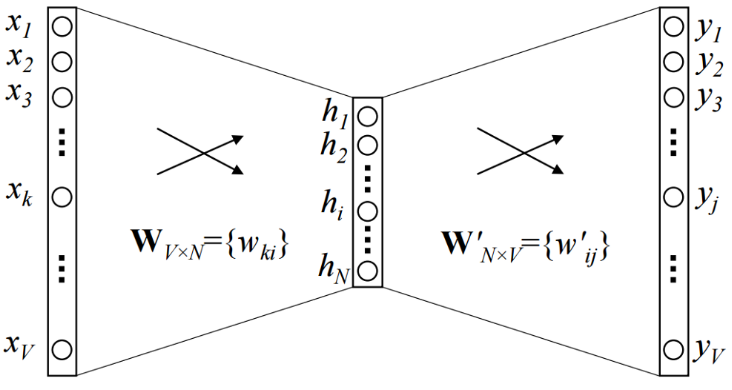
\includegraphics[width=0.75\linewidth]{screenshot002}
	\caption{Простая CBOW модель с одним словом в контексте, где
		\newline		 $x = \left\{ 	\begin{array}{l}
				x_{1} \\
				\dots \\
				x_{V}
			\end{array}
		\right\}
$ -- слой входных данных, 
	\newline		 $h = \left\{ 	\begin{array}{l}
		h_{1} \\
		\dots \\
		h_{N}
	\end{array}
	\right\}
$ -- скрытый слой,
	\newline		 $y = \left\{ 	\begin{array}{l}
		y_{1} \\
		\dots \\
		y_{V}
	\end{array}
	\right\}
$ --  слой выходных данных, 
	\newline
	$\mathbf{W}_{V \times N}=\left\{w_{k i}\right\}$ — весовая матрица, которая отображает входной слой $x$ в скрытый слой $h$,
	\newline
	$\mathbf{W}_{N \times V}^{\prime}=\left\{w_{i j}^{\prime}\right\}$ -- 
	весовая матрица, которая сопоставляет выходные данные скрытого слоя с конечным выходным слоем.
 }
	\label{fig:screenshot001}
\end{figure}



Вход или контекстное слово представляет собой один горячий закодированный вектор размера V. Скрытый слой содержит N нейронов, на выходе снова представляет собой вектор длины V, элементы которого являются softmax-значениями.

Нейроны скрытого слоя данной архитектуры просто копируют взвешенную сумму входных данных на следующий слой и не используют классические функции активации (такие как сигмоидная, $\tanh$ или ReLU). Нелинейность вводится за счет вычисления softmax в выходном слое.

В приведенной выше архитектуре модели для предсказания целевого слова использовалось одно контекстное слово. 
Рассмотрим архитектуру модели, где на входе может использоваться  несколько контекстных слов, представленную на Рисунке ниже.

\begin{figure}[H]
	\centering
	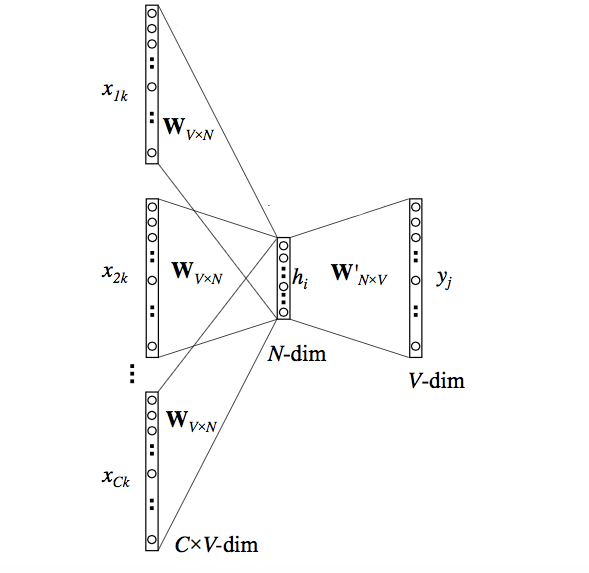
\includegraphics[width=0.7\linewidth]{screenshot003}
	\caption{Архитектура CBOW модель с  $C$ словами в контексте, где
			\newline		 $x_{i} $ -- слой входных данных из контекстного слова $i=1,\dots,C$, 
			\newline		 $h $ -- скрытый слой,
			\newline		 $y
$ --  слой выходных данных, 
			\newline
			$\mathbf{W}_{V \times N}=\left\{w_{k i}\right\}$ — весовая матрица, которая отображает входные слои $x$ в скрытый слой $h$,
			\newline
			$\mathbf{W}_{N \times V}^{\prime}=\left\{w_{i j}^{\prime}\right\}$ -- 
			весовая матрица, которая сопоставляет выходные данные скрытого слоя с конечным выходным слоем.}

	\label{fig:screenshot003}
\end{figure}



Данная архитектура использует $C$  контекстных  слов. Матрица $\mathbf{W}_{V \times N}$  используется для вычисления входных данных скрытого слоя. Для этого расчитывается среднее значение для всех $C$ входных контекстных  слов. 

Вторым способом создания вложения слов (word embedding) является моделью Skip-Gram, в которой целевое слово,  представление которого необходимо  сгенерировать, используется  для предсказания его контекста, в процессе чего и создается представление слова в векторном виде. 

Ниже на Рисунке представлена архитектура модели Skip-Gram, которая в значительной степени напоминает перевернутую модель CBOW с несколькими контекстными словами.


\begin{figure}
	\centering
	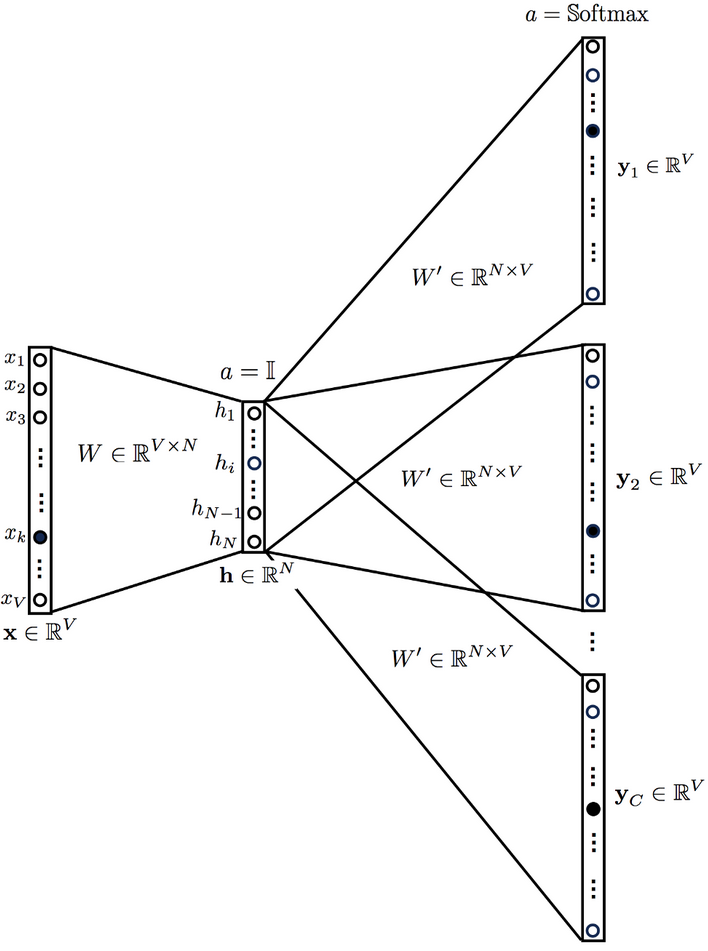
\includegraphics[width=0.7\linewidth]{screenshot004}
	\caption{Архитектура Skip-Gram модели  с  $C$ словами в контексте, где
	\newline		 $x$ -- слой входных данных из  целевого слова
	\newline		 $h $ -- скрытый слой,
	\newline		 $y
$ --  слой выходных данных для 	контекстных слов $i=1,\dots,C$, 	
	\newline
	$\mathbf{W}_{V \times N}=\left\{w_{k i}\right\}$ — весовая матрица, которая отображает входной слой $x$ в скрытый слой $h$,
	\newline
	$\mathbf{W}_{N \times V}^{\prime}=\left\{w_{i j}^{\prime}\right\}$ -- 
	весовая матрица, которая сопоставляет выходные данные скрытого слоя с конечными  выходными  слоями.}
	\label{fig:screenshot004}
\end{figure}

На входе модели Skip-Gram вводится целевое слово. В результате модель выводит $C$  распределений вероятностей, т. е. для каждого контекстного слова получается  $C$  распределений вероятностей из $V$  вероятностей, по одной для каждого слова.

В обоих случаях для обучения нейронной  сети  использует метод обратного распространения ошибки (backpropagation).
Оба метода имеют свои преимущества и недостатки. С одной стороны Skip Gram лучше работает с небольшим объемом данных и хорошо отображает редкие слова.
С другой стороны, CBOW быстрее и лучше отображает более часто встречающиеся слова.
Также, отметим, что  чтобы сделать алгоритм более эффективным в вычислительном отношении, используются такие приемы, как Hierarchical Softmax и Skip-Gram Negative Sampling. 


С тех пор, как был предложен метод  word2vec, появилось много расширений, включая GloVe \footnote{J. Pennington, R. Socher, and C. D. Manning, “Glove: Global 	vectors for word representation,” in EMNLP, 2014, pp. 1532–1543.}, улучшающий  векторы слов за счет учета глобальной статистики корпуса, и Doc2Vec \footnote{Q. V. Le and T. Mikolov, “Distributed representations of sentences 	and documents,” in ICML, 2014, pp. 1188–1196.}, генерирующий векторные  представления документов. 

Еще одним методом получения скрытой семантики является моделирование скрытой темы (или тематическое моделирование). Например, популярным является применение   модели Латентного  размещение Дирихле (Latent Dirichlet allocation, LDA)\footnote{D. M. Blei, A. Y. Ng, and M. I. Jordan, “Latent dirichlet allocation,” Journal of Machine Learning Research, vol. 3, pp. 993–1022, 	2003.} представляющего собой генеративную модель, которую можно использовать для объяснения сходства определенных частей наборов данных с использованием ненаблюдаемых групп. 

LDA — это одна из моделей «тематического  моделирования», по сути являющаяся это генеративной  моделью, которая позволяет объяснять  с помощью ненаблюдаемых или скрытых переменных,  почему некоторые части данных похожи или потенциально относятся к группам сходных «тем». 
Первоначально модель была представлена  в виде  графической модели, оцениваемой  с использованием методов вариационного вывода. 

Целью применения данной модели является описание объекта, с помощью вектора весов относящих его к различным темам. Например, текст о Великой депрессии можно представить с помощью следующего  вектора весов: экономика --  60\%, история Америки -- 30\% и  социальные проблемы  -- 10\%.  После получения вектора весов  можно использовать полученные меры расстояния для сравнения объекта в «тематическом» пространстве, а похожие объекты, например,  могут  быть получены на основе методов «ближайших соседей». 


Две основные части генеративной модели LDA -- это

\begin{enumerate}
	\item Набор «тем» или распределений по «словам»
	\item Для каждого «документа» распределение  по темам 
\end{enumerate} 


Опишем подробнее  генеративный процесс для LDA. Для каждого документа сгенерировать  распределение по $D$ темам $\theta_{d}$, причем распределение имеет вид 

$$
\theta_{d} \sim \operatorname{Dirichlet}(\alpha), d=1, \ldots, D, 
$$

где  $\alpha$ -- параметр распределения Дирихле.

Для $n$-го слова в $d$-м документе тема слова $z_{d n}$ выбирается из распределения 

$$
z_{d n} \sim D i \operatorname{screte}\left(\theta_{d}\right).
$$ 

После чего генерируется  слово $w_{d n} $ из выбранной темы $z_{d n}$, 

$$
w_{d n} \sim P\left(w_{d n} \mid z_{d n}, \beta\right),
$$

где $\beta$ является  матрицей размерности $K \times|W|$ с элементами, которые определяются как
$$
\beta_{i j}=p\left(w^{j}=1 \mid z^{i}=1\right).
$$ 


Байесовская модель для LDA требует алгоритма вывода для изучения апостериорного распределения параметров по заданным данным. 
На входе известны  только данные, распределения по темам, работам, темам, показателям и т. д. --  неизвестные параметры модели. 


На Рисунке ниже представлено графическое представление модели LDA:

\begin{figure}[H]
	\centering
	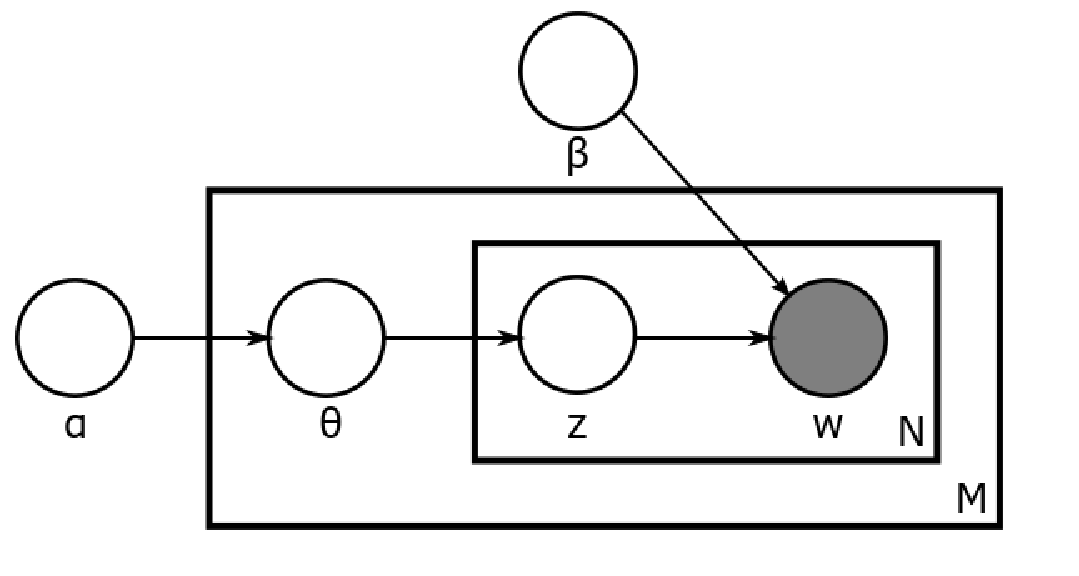
\includegraphics[width=0.7\linewidth]{screenshot005}
	\caption{Графическое представление модели LDA}
	\label{fig:screenshot005}
\end{figure}

Из данного графического представления можно получить следующую функцию совместного распределения:
$$
P(\theta, Z, W \mid \alpha, \beta)=p(\theta \mid \alpha) \prod_{n=1}^{N} p\left(z_{n} \mid \theta\right) p\left(w_{n} \mid z_{n}, \beta\right)
$$

где 

$\theta$ -- вектор тем в документе,

$Z$ -- вектор тем слов,

$W$ -- вектор слов, 

$\alpha$ -- параметр распределения Дирихле,

$\beta$ -- матрица размерности $K \times|W|$,

$z_{n}$ -- выбранная тема слова, 

$w_{n}$ -- сгенерированное слово.


В рамках сглаженная LDA модели (Smoothed LDA Model)
распределение Дирихле может  быть  дополнительно  размещено на распределении слов по заданной теме, с целью получения более робастного  решения. Такой поход также помогает получить распределение, которое  сконцентрировано вокруг точек, отражающих  релевантные слова. 


Генеративный процесс для сглаженного LDA можно представить следующим образом. Во-первых каждая  тема, представляется в виде распределения по $K$ словам $\varphi_{k}$

$$
\varphi_{k} \sim \operatorname{Dirichlet}(\beta), k=1, \ldots, K
,
$$

где $\beta$ -- параметр распределения Дирихле.
 

Для каждого документа формируется распределение по $D$ темам  $\theta_{d}$

$$
\theta_{d} \sim \operatorname{Dirichlet}(\alpha), d=1, \ldots, D,
$$

где $\alpha$ -- параметр распределения Дирихле.


Для $n$-го слова в $d$-м документе выбирается тема для слова $z_{d n} $

$$
z_{d n} \sim \operatorname{Discrete}\left(\theta_{d}\right)
$$

После чего слово $w_{d n}$ из выбранной темы $z_{d n} $, можно сгенерировать с помощью

$$
w_{d n} \sim \operatorname{Discrete}\left(\varphi_{z_{d n}}\right).
$$


Графическое представление модели сглаженного LDA можно отразить в виде схемы на Рисунке ниже. 

\begin{figure}[H]
	\centering
	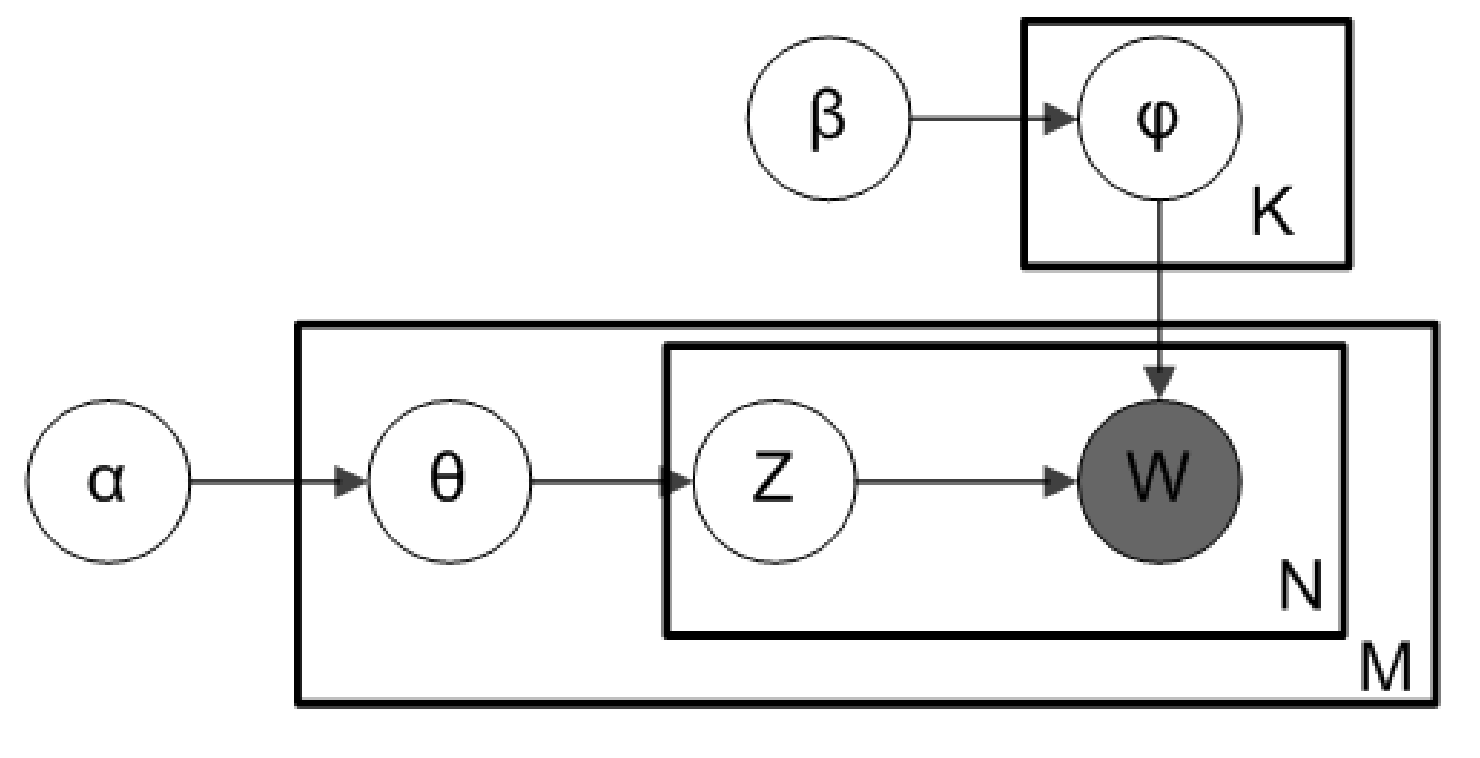
\includegraphics[width=0.7\linewidth]{screenshot006}
	\caption{Графическое представление модели сглаженного LDA}
	\label{fig:screenshot006}
\end{figure}


Распределение Дирихле имеет плотность вероятности, представляемой в виде 

$$
p(\theta \mid \alpha)=\frac{\Gamma\left(\sum_{i=1}^{k} \alpha_{i}\right)}{\prod_{i=1}^{k} \Gamma\left(\alpha_{i}\right)} \theta_{1}^{\alpha_{1}-1} \ldots \theta_{k}^{\alpha_{k}-1}
$$


где $\alpha$ -- параметр распределения Дирихле, являющийся  вектором размерности $k$ с компонентами $\alpha_{i}>0$,

$\Gamma(x)$  -- гамма-функция. 

Причем

$$
\mathbb{E}\left(\theta_{i}\right)=\frac{\alpha_{i}}{\sum \alpha_{i}}
.
$$

Распределение Дирихле — непрерывное распределение вероятностей  над полем  дискретных  распределений вероятностей. 
В зависимости от выбора распределения вектора параметров  $\alpha$    может отдавать предпочтение разреженным дискретным вероятностям по  $k$  темам, причем высокие значения параметров векора $\alpha$  позволяют присвоить  больше тем на документ, и наоборот. 
Для $k = 2$  распределение  Дирихле сводится  к бета-распределению. 


Таким образом для постановка проблемы имеется 
\begin{itemize}
	\item известный вектор  «слов» $W$,
	\item неизвестная матрица распределение объектов  по темам   $\beta$  размерности $K \times|W|$,
	\item скрытая переменная $Z $ распределения тем на слово,
	\item скрытая переменная $\theta$ распределения тем на документ.
\end{itemize}  

Две скрытые переменные масштабируются относительно  размерности  входных данных, где $\beta$  -- матрица фиксированной размерности. Для вывода скрытых переменных требуется вычисление апостериорной вероятности: 

$$
p(\theta, z \mid w, \alpha, \beta)=\frac{p(\theta, z, w \mid \alpha, \beta)}{p(w \mid \alpha, \beta)}
$$

Однако, стоит отметить, что невозможно рассчитать  знаменатель данной функции. Для вывода обычно используются два основных подхода:

\begin{itemize}
	\item Вариационный вывод с помощью EM-алгоритма, преимуществом которого является скорость вычисления.
	\item Сэмплирование по Гиббсу с помощью алгоритма MCMC, преимуществом которого является точность  вычислений.	
\end{itemize}

В рамках вариационного вывода используется упрощающее предположение для апостериорного распределения  основе. В этом случае импользуется предположение «среднего поля», т. е. каждая скрытая переменная контролируется своей собственной вариационной переменной, определяющей класс возможных приближенных апостериорных значений $q$:

$$
q(\theta, z \mid \gamma)=q\left(\theta \mid \gamma_{\theta}\right) \prod_{n=1}^{N} q\left(z_{n} \mid \gamma_{n}\right).
$$

Далее алгоритм вычисления $\gamma$ разрабатывается  таким образом, чтобы минимизировать расстояние Кульбака-Лейблера (KL-divergence), что эквивалентно  максимизации  доказательной или вариационной  нижней граница (Evidence lower bound, ELBO) для $q$ относительно истинного апостериорного $p$ как функции от  $\gamma$.

Нижняя доказательная граница (ELBO) задается как:

$$\log p(w \mid \alpha, \beta)=L(\gamma ; \alpha, \beta)+K L(q, p)$$

где 

$$
L(\gamma ; \alpha, \beta)=\mathbb{E}_{q}[\log P(\theta, z, w \mid \alpha, \beta)]-\mathbb{E}_{q}[\log q(\theta, z)].
$$


EM-алгоритм  реализуется  до тех пор, пока ELBO не сойдется:

\begin{itemize}
	\item E-шаг алгоритма -- вычисление  $\gamma$  для каждого документа,
	\item  M-шаг алгоритма  -- для фиксированного $\gamma$   максимизируется  нижняя  граница  логарифма правдоподобия для $p(w \mid \alpha, \beta)$, что соответствует максимальному правдоподобию при приблизительном апостериорном распределении, полученном на Е-шаге алгоритма. 
\end{itemize} 

Решения для E и M  шагов получаются итеративно путем взятия производных от ELBO по соответствующим переменным.

При использовании метода сэмплирования по Гиббсу 
$\beta$  также может рассматриваться как скрытая переменная.
Совместные апостериорные распределения 
$$
p(\beta, \theta, z \mid w) \sim\{\text { GibbsSample }\}
$$ 
получаются путем сэмплирования по Гиббсу. 
Поиск начинается  с начальных предположений для параметров модели $\beta, \theta, z$  и продолжается пока не будут  перебраны  все релевантные значения по каждой переменной.

При использовании алгоритма «свернутой» выборка Гиббса путем аналитической маржинализации переменных можно  уменьшить  число распределений для сэмплирования  до единственной скрытой переменной 
$z \sim p(z \mid w)$. 
В таком случае $\theta$ и $\beta$  восстанавливаются с помощью  математического ожиданий над $p(z \mid q)$. 
Такой метод работает намного быстрее, чем обычный алгоритм сэмплирования  по Гиббсу, и фактически быстрее  метода вариационного вывода, использующего EM алгоритм. К тому же, данный метод позволяет использовать небольшие наборы данных.

Следующим способом сбора данных является аугментация данных. Во многих случаях наборы данных являются неполными и должны быть заполнены путем сбора дополнительной информации. Отсутствующая информация может быть представлена как отдельными значениями, как и отдельными признаками. В качестве одного из способов аугментации данных можно рассмотреть интеграцию  данных.
На практике многие компании используют реляционные базы данных, в которых обучающие данные разделены на меньшие таблицы. Однако большинство инструментов машинного обучения предполагают, что обучающий набор данных представляет собой один файл, и игнорируют тот факт, что обычно в базе данных имеется несколько таблиц.
Ключевой вопрос заключается в том, полезно ли объединение таблиц и дополнение информации для обучения модели.\footnote{A. Kumar, J. F. Naughton, J. M. Patel, and X. Zhu, “To join or not 	to join?: Thinking twice about joins before feature selection,” in 	SIGMOD, 2016, pp. 19–34.} 

Также к одному из методов сбора данных можно отнести генерацию  данных, которая используется в случае, когда нет доступных существующих наборов данных, которые можно было бы использовать для обучения модели,. Для ручной генерации данных используется краудсорсинг — стандартный метод, когда людям даются задания по сбору необходимых данных. В качестве альтернативы можно использовать автоматические методы для создания синтетических наборов данных. 
Генерацию данных с помощью краудсорсинга можно разделить на два этапа: сбор данных и предварительная обработка данных. 


В настоящее время генерация синтетических данных все чаще используется в машинном обучении из-за низкой стоимости и гибкости  метода \footnote{N. Patki, R. Wedge, and K. Veeramachaneni, “The synthetic data 	vault,” in DSAA, 2016, pp. 399–410.}. 

Простой метод заключается в том, чтобы выбрать параметры  начального распределения вероятностей и сгенерировать выборку из этого распределения, например,  с помощью  инструментов из пакета scikitlearn. 

Кроме того, существуют более продвинутые методы, такие как генеративно-состязательные сети (GAN)\footnote{I. J. Goodfellow, J. Pouget-Abadie, M. Mirza, B. Xu, D. Warde-Farley, S. Ozair, A. Courville, and Y. Bengio, “Generative adver	sarial nets,” in NIPS, 2014, pp. 2672–2680.}. Далее будут кратко описаны модели генеративно-состязательные сети (GAN). 

Ключевым  подход GAN заключается в обучении двух конкурирующих нейронных сетей: генеративной сети и дискриминационной сети. Генеративная сеть учится сопоставлять скрытое пространство с распределением данных, а дискриминативная сеть отличает примеры истинного распределения от кандидатов, созданных генеративной сетью.

Обучение GAN можно формализовать следующим образом:

$$
\begin{array}{c}
	\min _{G} \max _{D} V(D, G) \\
	V(D, G)=\underset{x \sim p_{\text {data }}(x)}{\mathbb{E}}[\log D(x)]+\underset{z \sim p_{z}(z)}{\mathbb{E}}[\log (1-D(G(z))]
\end{array}
$$


где  $p_{\text {data }}(x)$ ) — распределение реальных данных,

$p_{z}(z)$  — распределение генератора, 

$G(z)$ --  порождающая сеть, 

$D(x)$  --  дискриминационная сеть. 


Целью генерирующей сети является увеличение частоты ошибок дискриминационной сети. Другими словами, генерирующая сеть пытается обмануть дискриминационную сеть, заставляя ее думать, что ее кандидаты из истинного распределения. 

GAN были использованы для генерации реалистичных синтетических изображений и видео во многих приложениях. В настоящее время GAN также были использованы  для создания синтетических реляционных данных. Так, например  medGAN\footnote{E. Choi, S. Biswal, B. Malin, J. Duke, W. F. Stewart, and J. Sun, 	“Generating multi-label discrete patient records using generative 	adversarial networks,” in MLHC, 2017, pp. 286–305} генерирует синтетические записи пациентов с многомерными дискретными  (двоичными или счетными) признаками  на основе реальных записей пациентов. 

В то время как GAN могут только аппроксимировать отдельные записи пациентов, одним из новейших способов генерации данных является  использование  автокодировщиков для проецирования этих записей в пространство более низкого измерения, с последующей их декаодировкой -- проецированием  их обратно в исходное пространство.

 
Модель TABLE-GAN \footnote{N. Park, M. Mohammadi, K. Gorde, S. Jajodia, H. Park, and 	Y. Kim, “Data synthesis based on generative adversarial networks,” PVLDB, vol. 11, no. 10, pp. 1071–1083, 2018.} позволяет  синтезировать  таблицы, похожие на настоящие  с упором на сохранение конфиденциальности. В частности в таких моделях, определяется  метрика потери информации и два параметра для корректировки потери информации. Чем выше потери, тем больше конфиденциальности у синтетической таблицы.


Следующим блоком сбора данных в рамках моделей машинного обучения является разметка данных. 
Во многих случаях сбор данных выполняется одновременно с разметкой  данных. Можно выделить следующие категории методов разметки данных\footnote{https://arxiv.org/pdf/1811.03402.pdf}:

\begin{itemize}
	\item  Использование существующих меток: первоначальная идея разметки данных заключалась в использовании любых уже существующих меток. Существует обширная литература по полуавтоматическому обучению, идея которого  состоит в том, чтобы учиться на уже существующих  метках предсказывать остальные метки. 
	\item  Краудсорсинг: простые  подходы состоят в том, чтобы пометить отдельные примеры, более продвинутые используют методы активного обучения, при котором вопросы, которые  задаются разметчику данных, выбираются более тщательно. 
	\item  Методы слабой разметки: не смотря на то, что желательно постоянно генерировать правильные метки, этот процесс может быть слишком дорогим. Альтернативный подход состоит в том, чтобы заново генерировать менее совершенные метки (т. е. слабые метки), но в больших количествах, чтобы компенсировать более низкое качество самих меток. Именно этот метод в последнее время набирает все большую популярность, поскольку во многих новых приложениях мало размеченных данных.
\end{itemize} 

Каждый подход к маркировке можно дополнительно разделить на следующие категории: 

\begin{itemize}
	\item  Задачи машинного обучения. 
	
	В  обучении с учителем есть две категории:   классификация (например, определение того, имеет ли фрагмент текста положительное настроение) и регрессия (например, оценка заработной платы работника). Большая часть исследований по маркировке данных была сосредоточена на проблемах классификации, а не на проблемах регрессии, возможно, потому, что маркировка данных проще в рамках моделей классификации. 
	
	\item  Тип данных. 
	
	В зависимости от типа данных (например, текст, изображения и графики) методы маркировки данных существенно различаются. Например, извлечение фактов из текста сильно отличается от обнаружения объектов на изображениях. 
\end{itemize}


Часто  задача машинного  обучения состоит в том, чтобы получить с помощью   небольшой объем размеченных данных метки для  гораздо большего  объема неразмеченных данных. 
Методы полуавтоматического обучения\footnote{X. Zhu, “Semi-Supervised Learning Literature Survey,” Computer Sciences, University of Wisconsin-Madison, Tech. Rep.} 
используют как размеченные, так и неразмеченные данные для прогнозирования. 


Для методов полуавтоматического обучения,  применяемых   для классификации,  цель состоит в том, чтобы обучить модель, которая возвращает один из нескольких возможных классов для каждого примера с использованием как размеченных, так и неразмеченных наборов данных.

Простейший класс методов полуавтоматического обучения обучает одну модель с использованием одного алгоритма обучения на одном наборе признаков. Например, самообучение\footnote{D. Yarowsky, “Unsupervised word sense disambiguation rivaling 	supervised methods,” in ACL, 1995, pp. 189–196.} изначально обучает модель на помеченных примерах. Затем модель применяется ко всем неразмеченным данным, где примеры ранжируются по достоверности их прогнозов. Затем наиболее достоверные прогнозы добавляются к размеченным примерам.
Этот процесс повторяется до тех пор, пока не будут выбраны метки для всех   неразмеченных примеров. 

Следующий класс моделей  обучает несколько классификаторов, несколько раз отбирая обучающие данные и обучая модель для каждой выборки. Например, Tri-обучение \footnote{Z.-H. Zhou and M. Li, “Tri-training: Exploiting unlabeled data 	using three classifiers,” IEEE TKDE, vol. 17, no. 11, pp. 1529–1541, Nov. 2005} изначально обучает три модели на размеченных примерах, используя бэггинг для алгоритма обучения ансамбля. Затем каждая модель интеративно обновляется, когда две другие модели делают прогнозы на неразмеченных примерах, и только примеры с одинаковыми прогнозами используются в сочетании с исходными размеченными примерами для повторного обучения модели.
Процесс останавливается, когда модель перестает изменяться. В итоге, неразмеченные примеры помечаются с использованием голосования большинством, при котором по крайней мере две модели должны согласовываться друг с другом.


Относительно меньше исследований было проведено в отношении полуавтоматического обучения для регрессии, целью которого является обучение модели, предсказывающей действительное число по примеру. Например, ко-регуляризованная регрессия, оцененная   методом наименьших квадратов  (МНК)\footnote{U. Brefeld, T. G ̈artner, T. Scheffer, and S. Wrobel, “Efficient co-regularised least squares regression,” in ICML, 2006, pp. 137–144.} представляет собой алгоритм оценки регрессии методом наименьших квадратов, основанный на подходе совместного обучения. 

Другая совместно структура основанна на использовании двух    регрессоров  совместного  обучения \footnote{Z.-H. Zhou and M. Li, “Semi-supervised regression with co-training,” in IJCAI, 2005, pp. 908–913.},  получаемых по методу $k$-ближайших соседей с разными метриками расстояния. На каждой итерации регрессор помечает неразмеченные данные, которые с наибольшей вероятностью могут быть помечены вторым регрессором. После завершения итеративного процесса  окончательный прогноз примера делается путем усреднения оценок, полученной по  этим двум регрессорам. 

Также, один из классов моделей разметки данных в включает в себя методы распространения меток на основе графов, который  также начинает итеративный процесс с ограниченного набора помеченных примеров, но для получения меток для остальных наблюдений  используют структуру графа на основе их сходства. 

Часто при использовании моделей машинного  обучения, в большинстве случаев размеченных данных не хватает. В результате популярность набирают методы слабого обучения, идея которого  состоит в том, чтобы полуавтоматически генерировать большое количество меток, которые не так точны, как ручные метки, но достаточно хороши, чтобы обученная модель могла достичь  достаточно высокой точности. Этот подход особенно полезен, когда имеются большие объемы данных, и ручная разметка становится невозможной. 

Одним из методов слабой разметки данных является программирование данных. Для разметки используются ансамбли функций маркировки.   Поскольку одна функция маркировки сама по себе может быть недостаточно точной или неспособной генерировать метки для всех примеров, несколько функций маркировки реализуются и объединяются в генеративную модель, которая затем используется для создания большого количества слабых меток приемлемого качества. 
Для объединения функций маркировки можно также  использовать голосование большинством. Наконец, дискриминационная  модель обучается на слабых метках с учетом шума в данных. 


Другим способом создания слабых меток является использование метода  извлечения фактов. Базы данных часто  содержат факты, извлеченные из различных источников. Факт может описывать атрибут объекта и его можно использовать для формирования слабых меток. 


Последней группой методов рассматриваемой в рамках сбора данных с использованием моделей машинного обучения являются  методы улучшения имеющегося набора данных. 
Этот подход важен для широкого ряда сценариев. 

\begin{itemize}
	\item Во-первых, может быть сложно найти новые наборы данных, потому что приложение слишком новое, нетривиальное или специфическое.
	\item  Во-вторых, простое добавление дополнительных данных уже не может существенно повысить точность модели. 
\end{itemize}

В таком случае переразметка   или очистка существующих данных может быть наиболее быстрым способом повышения точности модели. В качестве альтернативы обучение модели можно сделать более устойчивым к шуму и систематическим  ошибкам, или модель можно обучить на основе существующей модели с использованием методов трансфертного обучения. 


Основная проблема машинного обучения заключается в том, что данные могут быть зашумлены, а изначальные метки расставлены  неправильно. 
В обоих  случаях, как,  если метки также зашумлены, так и, если метки неправильны, возникает необходимость в   переразметке наблюдений. 

В случае, если данные являются зашумленными, например, если некоторые значения могут быть вне допустимого диапазона  или по ошибке используются неверные  единицы измерения, необходимо использовать методы, позволяющие улучшить качество данных. 
Существуют системы различные системы очистки данных. Один из популярных фреймворков\footnote{ S. Krishnan, J. Wang, E. Wu, M. J. Franklin, and K. Goldberg, 	“Activeclean: Interactive data cleaning for statistical modeling,” PVLDB, vol. 9, no. 12, pp. 948–959, 2016.}, основан на том, что в нем итеративно предлагаются  образцы данных для очистки в зависимости от того, насколько очистка улучшает точность модели и оцененной вероятности  того, что данные являются шумом. Данная система рассматривает обучение и очистку как форму стохастического градиентного спуска и использует модели с  выпуклыми функциями  потерь (SVM, линейная и логистическая регрессия), чтобы гарантировать  наличие глобального экстремума для модели очищенной от шума. 

Другой фреймворк \footnote{S. Krishnan, M. J. Franklin, K. Goldberg, and E. Wu, “Boostclean: 	Automated error detection and repair for machine learning,” 	CoRR, vol. abs/1711.01299, 2017.} устраняет  классы несоответствий, когда значение атрибута находится за пределами разрешенного домена. Данная модель принимает на входе набор данных и набор функций, которые могут обнаруживать  ошибки  в данных и корректировать функции поиска ошибок. 
Каждая пара функций обнаружения и корректировки может породить  новую модель, обученную на очищенных данных. Для того,  чтобы найти наилучший набор пар функций, который максимизирует точность конечной модели в рамках этой модели используется статистический бустинг. 


Также в работе \footnote{V. S. Sheng, F. Provost, and P. G. Ipeirotis, “Get another label? 	improving data quality and data mining using multiple, noisy 	labelers,” in KDD, 2008, pp. 614–622.} было показано, что если метки зашумлены, то начиная с некоторой точки   точность модели выходит на плато и далее  не  увеличивается, независимо от того, сколько меток добавляется дополнительно. Для решение этой проблемы предлагается улучшить качество существующих этикеток. Причем в данной работе показывается, что переразметка с использованием рабочих характеристик меток  с определенными индивидуальными качествами может значительно повысить точность модели. 

Помимо улучшения данных, существуют также способы улучшить саму   модель, которая обучается. Повышение устойчивости обучения модели к шуму или систематической ошибке является активной областью исследований. Другой популярный подход заключается в использовании трансферного обучения, при котором ранее обученные модели используются в качестве отправной точки для обучения текущей модели. 

Часто простое отбрасывание зашумленных меток приводит к значительному  сокращению обучающих данных, что нежелательно для сложных моделей. Для того, чтобы модели могли   использовать  зашумленные метки, став более робастными к шуму в данных, могут использоваться сверточные нейронные сети, обученные на наборах данных  с небольшим количеством чистых меток и большим количеством зашумленных меток. Идея состоит в том, чтобы смоделировать отношения между объектами, метками классов и шумами меток с помощью вероятностной модели и впоследствии интегрировать ее в обучение основной модели.  
В рамках такой модели шумы подразделяются  на два типа: шумы,    вызванные, тем, что категории перепутаны между собой, и чисто случайные шумы, вызванный техническими ошибками, такими как несоответствие между объектом и контекстом. Истинные метки и типы шума рассматриваются как скрытые переменные, и для статистическго вывода используется EM-алгоритм. 


Также, для улучшения самой модели может использоваться трансферное обучение. Трансферное обучение  — это популярный подход к обучению моделей, который применяется,  когда не хватает обучающих данных или времени для обучения с нуля. Данный  метод заключается в том, чтобы начать с существующей модели, которая хорошо обучена (исходной задачи), после чего  можно постепенно обучать новую модель (целевую задачу), которая уже хорошо работает. 
Например, одни сверточные нейронные сети могут использоваться для обучения другой модели используемой для смежной  проблемы. 
В дополнение к использованию предварительно обученных моделей другой популярный метод заключается в  обучении за несколько шагов. 
Существуют также исследования методов трансферного обучения в контексте нейро-лингвистического  программирования, компьютерного зрения и глубокого обучения.

Индуктивное трансферное обучение используется, когда исходная задача и целевая задача различаются, а две области могут быть или не быть одинаковыми. Здесь задачей может быть категоризация документа, в то время как домен может быть набором университетских веб-страниц для классификации.
Трансдуктивное трансферное обучение используется, когда исходная и целевая задачи одинаковы, но домены разные. 


Итак, по мере того, как машинное обучение становится все более популярным, все важнее становятся методы сбора больших объемов  данных и способы  их разметки, особенно в контексте их применения к современным  нейронным сетям. Традиционно для  решения этой проблемы использовались методы обработки естественного языка и компьютерного зрения. В первую очередь эти методы применялись  для разметки данных. Сегодня для решения многочисленных подзадач, связанных со сбором, разметкой и улучшением существующих данных, было создано множество специфических методов, основанных на применении широкого спектра моделей машинного обучения, дополняющих  друг друга. 


\section{Методология обработки  данных}


В данном разделе будут подробнее рассмотрены основные способы предварительной  обработки  данных. Независимо от источника набора данных, который используется  для создания системы машинного обучения, этот же набор данных необходимо уточнить, предварительно обработать и заполнить пропуски.

Предварительная обработка данных — это сложный термин, который отражает совокупность множества действий, начиная от форматирования данных и заканчивая созданием комбинированных признаков, которые в последствие могут подаваться на входе для выбранной модели. При анализе набора данных, например на наличие  дисбаланса среди подклассов, можно учитывать распределение данных среди этих классов; или если известны, какие признаки  являются необзательными или нерелевантными для анализа, то уже на этом этапе можете снизить  размерность набора данных. 

Ниже  будут перечислены, существующие  подходы для эффективной предварительной обработки данных.

\begin{enumerate}
	\item  Форматирование данных

В большинстве случаев после этапа сбора данных имеется набор данных, полученный  из различных источников, для которых  способы  хранения и представления различны. Часто окончательный набор данных представляет собой файл CSV или собирается из других файлов типа XLS/CSV или экспортированных электронных таблиц из внешних баз данных. Следовательно перед обработкой данных необходимо свести всю имеющуюся информацию в одну таблицу, приведя данные к одному виду.

\item  Очистка данных

Форматированные данные — это данные в том формате, в котором их можно подать ML-фреймворку. Однако, данные могут иметь ошибки,  выбросов (аномалии) и пропуски. Наличие этих проблем может повлиять на финальный результат, поэтому важна предварительная очистка данных перед дальнейшей обработкой. 
Наиболее частыми проблемами в данных можно назвать: 

\begin{itemize}
	\item отсутствующие или пропущенные данные: подходы, которые можно использовать для заполнения пропусков, зависят от типа отсутствующих данных (числовых или категориальных), так для числовых пропусков, например, можно использовать среднее значение, для категориальных – наиболее частое значение;
	\item дубликаты: очевидно, наличие повторяющихся наблюдений в наборе данных не имеет положительного влияния на точность  модели, а вариативность в данных, наоборот, напрямую на нее влияет;
	\item  структурные ошибки: к ним могут относиться опечатки или  ошибки в названиях классов;
	\item выбросы: наличие выбросов наиболее частая проблема в наборах данных, в большинстве моделей отсутствие выбросов  является одним из основных предположений, поэтому аномальные значения должны быть заранее отсортированы и удалены из набора данных, поскольку для работы с этими данными могут потребоваться  специально предназначенные для этого модели, отличающиеся от тех, которые должны применяться к подавляющему большинству данных;
	\item  агрегирование данных:  агрегирование может применяться к строкам и атрибутам данных с целью уменьшения набора  данных меньше для сокращения необходимого  времени и памяти для анализа данных на следующих этапах.
\end{itemize}

Если набор данных содержит много наблюдений, то можно сократить  количество наблюдений, с целью  удаления неполных или нерепрезентативных данных,  не  теряя  при этом в качестве. 


\item  Сэмплинг (выборка данных)

Это процесс выбора данных из генеральной совокупности (общего набора данных)  для анализа. Основная особенность создания выборки  состоит в том, что это выбранное подмножество данных должно быть репрезентативным и сбалансированным. На практике можно использовать метод  простой случайной выборки или  выборку с  повторениями.

\item  Разработка признаков 

Процесс формирования признаков включает в себя множество действий, многие  из которых взаимосвязаны с уже упомянутыми проблемами в данных и по определяются стоящей перед исследователем  задачей.

\item  Обработка категориальных данных

Признаки, которые могут принимать только определенные значения (например, штат, город,  цвет и т. д.), называются категориальными данными. Категориальные данные можно разделить на порядковые (значения, которые можно отсортировать или упорядочить, например, размер или качество) и номинальные (не подразумевают порядок, например, название региона) значения. Алгоритмы машинного обучения не работают со текстовыми данными, что означает, что необходимо заранее преобразовать текстовые значения в численные. Учитывая разницу между порядковыми и номинальными данными, преобразование должно производиться с сохранением смысла значений категориальных данных. Основными методами здесь будут сопоставление порядковых признаков, кодирования меток и фиктивных переменных.

\item  Масштабирование признаков

Цель этой процедуры — привести числовые признаки к одному масштабу. Часто алгоритмы машинного обучения могут в большей степени учитывать признаки с большими числовыми значениями, что  уменьшает  полезность признаков с малыми числовыми значениями. Для того, чтобы избежать потери информации, содержащейся в признаках с малыми числовыми значениями, применяются два распространенных подхода: нормализация и стандартизация данных.
Оба метода широко используются в машинном обучении  и иногда могут быть взаимозаменяемыми (в зависимости от выбранного алгоритма).

\item  Уменьшение размерности

Количество переменных или признаков в наборе данных машинного обучения определяет его размерность. Таким образом, уменьшение размерности означает процесс, состоящий из подходов или действий, которые уменьшат количество признаков. Слишком большое количество признаков  приводит к увеличению необходимого  объема памяти, используемого  для обработки данных, проблеме с переобучением и, так называемому,  проклятию размерности. Данный пункт иногда можно объединить с этапом выбора  признаков, однако основным отличием процесса уменьшения  размерности набора данных заключается в том, что  создается  новый набор признаков для объектов выборки, в то время как после процедуры выбора признаков создается набор данных из наиболее полезных из существующих признаков. 

\item  Выбор признаков 

Для выбора, наиболее  значимых и полезных из существующих признаков. используются  следующие методы.

\begin{itemize}
	\item Методы фильтрации:  признаки выбираются и ранжируются в соответствии с их вкладом в целевую функцию.
	\item  Методы свертки: поиск наиболее эффективных комбинаций признаков.
	\item Методы вложения: выбор признаков, которые больше всего способствуют производительности модели, который применяется во время  обучения модели.
	\item Создание признаков:  процесс и создание новых признаков, которые будут способствовать улучшению качетсва модели в большей степени, чем уже существующие. Данный процесс включает в себя множество действий, таких как сопоставление данных, дискретизация и уже упомянутое  выше масштабирование признаков. 
\end{itemize}

\end{enumerate}

Таким образом, основной целью предварительной  обработки данных и создания признаков является создание наиболее полного и репрезентативного  набора данных, состоящего   из наиболее ценных для модели признаков.


Очистка данных в большинстве случаев является необходимым условием разработки качественной прикладной модели  машинного обучения. В большинстве исследований очистка данных рассматривается как отдельный этап работы над моделью, проводимый без учета  его влияния на качество финальной модели машинного обучения. В некоторых случаях неправильно проведенная  очистка данных может снизить производительность моделей машинного обучения.
Рассмотрим подробнее наиболее популярные методы, позволяющие очистить данные от шумов и выбросов. 

Во-первых, рассмотрим модель  SampleClean\footnote{S. Krishnan et al. “SampleClean: Fast and Reliable Analytics on Dirty Data”. In: IEEE Data 	Eng. Bull. 38 (2015), pp. 59–75}. В рамках этой модели предлагается метод моделирования очищенных данных на основе выборки из необработанных данных. Наивный подход обработки данных может ухудшать качество модели, поскольку семантика выбросов и шумов в данных в значительной степени отличается от семантики "чистых" данных, поэтому в рамках этой работы использовался так называемый метода аппроксимированной обработки  запросов (Approximate
Query Processing, AQP). AQP-метод  состоит из двух шагов: во-первых, на шаге прямой оценки (Direct Estimate, DE)  случайным образом  выбирается  и очищается набор  из $k$ строк, а результат обучения возвращается независимо от наличия выбросов и шумов в данных. Данный шаг сам по себе может привести к некорректным результатам, когда доля зашумленных наблюдений в выбранном подмножестве преобладает. Чтобы избавиться от этого недостатка, применяется последующий  шаг коррекции, на котором производится повторное взвешивание выборки на основе вклада очищенных данных во весь набор данных.
С помощью такого подхода можно достичь равновесия, при котором приблизительный результат  ограничен доверительным интервалом, который может гарантировать получение надлежащего количества очищенных данных при моделировании. Кроме того, если исследователь хочет получить определенное количество очищенных  данных в финальном наборе, метод SampleClean предлагает размер выборки, рекомендованный для достижения желаемого уровня точности. Также с  помощью метода стохастического градиентного спуска можно  вычислить среднее значение преобразованных данных для конкретного набора из неочищенных данных.  

Во-вторых, можно использовать  метод  очистки данных под названием ActiveClean\footnote{Sanjay Krishnan et al. “Activeclean: An interactive data cleaning framework for modern machine 	learning”. In: Proceedings of the 2016 International Conference on Management of Data. 2016, 	pp. 2117–2120.}.  Модель ActiveClean, в отличие от SampleClean, создающей сгенерированную выборку из очищенных данных, позволяет сохранить изначальные данные в модели за счет использовния функций-оптимизаторов. Оптимизаторы — это алгоритмы стохастического  градиентного  спуска, которые итеративно отбирают данные, переоценивают градиент и обновляют текущую лучшую модель. 
Для применения  этого метода можно использовать даже небольшие наборы данных. 
Модель ActiveClean постепенно очищает набор данных, оценивая модели, использующие выпуклые функции потерь (например, логистическую  регрессию  или  машину опорных векторов (SVM)). Ключевое отличие заключается в том, что ActiveClean стремится постепенно очищать базовый набор данных, чтобы изучаемая  модель становилась более эффективной по мере получения большего количества очищенных записей. 

В-третьих, еще одна модель  очистки данных  была представлена в работе\footnote{Sanjay Krishnan et al. “Activeclean: An interactive data cleaning framework for modern machine 	learning”. In: Proceedings of the 2016 International Conference on Management of Data. 2016,	pp. 2117–2120.} под названием HoloClean. Основное отличие  этой модели  от других подходов заключается в том, что она учитывает предельную вероятность при рассмотрении наблюдения-кандидата на очистку. 
Авторами была  разработана  модель, которая учится как на чистых, так и на поврежденных данных, чтобы сделать вывод о том, где с высокой вероятностью могут возникнуть потенциальные ошибки. Далее предлагается обучить модель на относительно небольшой части реальных данных и проверить, может ли она сделать вывод о характере ошибок, допущенных при заполнении данных. Для обучения оптимальной модели HoloClean нужно большое количество как чистых, так и зашумленных наблюдений. Однако на практике часто сложно получить достаточное количество наблюдений данных из обеих категорий

В-четвертых, в работе \footnote{Sanjay Krishnan and Eugene Wu. “AlphaClean: Automatic Generation of Data Cleaning Pipelines”. In: (2019).}  была предложена система очистки данных AlphaClean, которая автоматизирует процесс поиска эффективного набора  инструментов очистки. Процесс создания функции очистки включает в себя выбор параметров для конкретного пайплайна. Модель AlphaClean позволяет  работать  с любым заданным количеством инструментов очистки. Данный метод строит комбинацию из функций очистки  в виде дерева. По мере продвижения алгоритма оптимальное решение становится постепенно доступным, а выходные данные пересматриваются на  дальнейших итерациях, что потенциально улучшает и  качество предлагаемой оптимальной комбинации функции очистки. Этот метод позволяет  оценивать результаты на каждой итерации, в частности, есть возможность  проверить, является ли предложенная комбинация функций очистки данных перспективной и следует ли ее рассматривать в качестве возможного оптимального решения. 

В-пятых, рассмотрим модель  CPClean, предложенную   в рамках модели классификации по методу  ближайших соседей при неполной информации \footnote{Bojan Karlaˇs et al. Nearest Neighbor Classifiers over Incomplete Information: From Certain 	Answers to Certain Predictions. 2020. arXiv: 2005.05117 [cs.LG]}.  Для изучения влияния наличия неполных данных на качество модели авторами было  предложено использование нескольких инструментов  проверки модели. 

Часто при работе с данными возникают ситуации, когда в обучающем наборе данных доля объектов одного из подкласса слишком мала. 
Слабо представленный в наборе данных класс будем называть миноритарным, и, наоборот,  наиболее часто встречающийся в наборе класс --  мажоритарным.
Ниже буду рассмотрены  методы ресэмплинга, используемые для борьбы с несбалансированными данными. 

Для борьбы с несбалансированностью наборов данных используют два основных подхода: 
\begin{itemize}
	\item Дублирование примеров миноритарного класса (Oversampling)
	\item Случайное удаление примеров мажоритарного класса (Undersampling) 
\end{itemize} 

Данные методы  используются для корректировки распределения классов в наборе данных, в частности набор данных пересобирается  таким образом, что соотношение между различными представленными классами/категориями становится более равномерным.

Как методы дублирования объектов миноритарного класса, так и метода удаления  примеров мажоритарного класса  предполагают искусственного  введения  систематической ошибки из-за  выбора большей доли наблюдений из одного класса, чем из другого, с целью компенсировать дисбаланс, который либо уже присутствует в данных, либо может возникнуть, если подвыборка из набора данных   будет формироваться с помощью метода простой случайной выборки. 

Дисбаланс в данных может быть следующих типов:
\begin{itemize}
	\item Недостаточная представленность какого-то класса в одной или нескольких важных переменных-предикторах. 
	\item Недостаточная представленность  какого-то   класса в выходной (зависимой) переменной. 
\end{itemize}

Как методы дублирования объектов миноритарного класса обычно используется чаще, чем методы  удаления  примеров мажоритарного класса, особенно когда подробные данные еще не собраны не полностью. 
Переизбыток данных стал проблемой только в эпоху «больших данных», а причины использования  методов  удаления  примеров мажоритарного класса  в основном связаны со  снижением необходимых  для оценки модели ресурсов (времени оценивания и необходимой памяти). 
В частности, для получения достоверных статистических выводов требуется достаточно большой размер выборки, причем  данные должны быть предварительно очищены. 



Рассмотрим подробнее методы дублирования объектов миноритарного класса. 
Во-первых, простейшим из подходом является метод случайного дублирования (Random oversampling). 
Случайная дублирование представляет собой метод дополнения набора данных несколькими копиями наблюдений, принадлежащих миноритарному  классу. Не смотря на простоту метода, данный метод является достоаточно надежным\footnote{Ling, Charles X., and Chenghui Li. "Data mining for direct marketing: Problems and solutions." Kdd. Vol. 98. 1998.}.   Объекты миноритарного класса могут быть полностью продублированы в новом наборе данных, либо могут быть выбраны с помощью метода простой случайной выборки с повторением.


Во-вторых, популярным подходом дублирования объектов является алгоритм синтетического дублирования SMOTE (Synthetic Minority Oversampling Technique). 
Алгоритм SMOTE для создания новых наблюдений использует интерполяцию  на пространстве признаков    между наблюдениями, которые находятся рядом.
В частности, сначала фиксируется   число наблюдений необходимых  для генерации $N$. Как правило, оно выбирается таким образом, чтобы распределение по бинарным классов в новом наборе данных было 1:1, однако распределение объектов по классам  может быть выбрано произвольным образом в зависимости от решаемой задачи и особенностей набора изначального данных. Алгоритм SMOTE  можно описать следущим образом: 
\begin{itemize}
	\item Итеративный процесс   начинается с выбора первого случайного наблюдения  экземпляра миноритарного класса.
	\item   Далее выбираются $k$  ближайших  соседей (обчынчо $k=5$) для этого наблюдения. 
	\item  После чего  $N$  из этих $k$  экземпляров выбирается для интерполяции новых синтетически сгенерированных наблюдений. Для этого с использованием любой метрики расстояния вычисляется разница в расстоянии между вектором признаков и его соседями. После чего полученная разница умножается на любое случайное значение в (0,1] и добавляется к предыдущему вектору признаков. 	
\end{itemize}

Результат работы алгоритма SMOTE представлен на Рисунке ниже.

\begin{figure}[H]
	\centering
	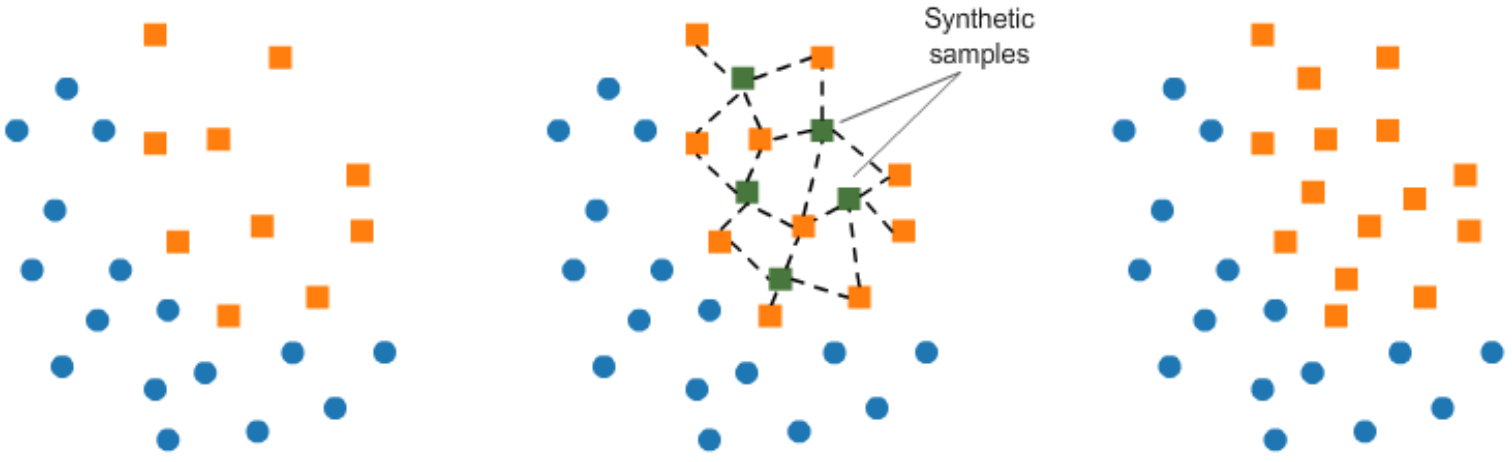
\includegraphics[width=1\linewidth]{screenshot007}
    \caption{Принцип работы алгоритма SMOTE. Источник:A Novel Resampling Technique for Imbalanced Dataset Optimization}
	\label{fig:screenshot007}
\end{figure}
Хотя этот алгоритм весьма полезен, он имеет несколько связанных с ним недостатков:

\begin{enumerate}
	\item Сгенерированные наблюдения расположены в одном направлении, т. е. соединены искусственной линией со своими диагональными соседями.
	\item SMOTE имеет тенденцию создавать большое число  зашумленных наблюдений на  пространстве признаков.
\end{enumerate}


В-третьих, еще одним популярным алгоритмом является алгоритм 
адаптивного  синтетического сэмплинга ADASYN (Adaptive synthetic sampling approach), 
который является обобщенной формой алгоритма SMOTE. Этот алгоритм дублирует объекты миноритарного класса путем создания новых синтетически сгенерированных наблюдений. Основным различием с алгоритмом SMOTE  является то, что ADASYN учитывает распределение плотности, $r_i$, которое определяет число наблюдений для генерации, которые трудно изучить. Благодаря этому ADASYN помогает адаптивно изменять границы решений на основе сложных для изучения образцов. 

Алгоритм ADASYN можно описать следующим образом:

\begin{enumerate}
	\item Из набора данных определяется общее число наблюдений мажоритарного  и миноритарного класса, $\mathbf{N}^{-}$ и $\mathbf{N}^{+}$,  соответственно. 
	\item  Устанавливается  пороговое значение $\mathbf{d}^{\text {th }}$  максимальной степени дисбаланса классов. 
	\item  Общее число синтетических наблюдений, которые необходимо сгенерировать определяется как
	
	$$
	G=\left(\mathrm{N}^{-}-\mathrm{N}^{+}\right) \times \beta
	$$
	
	где  $\boldsymbol{\beta}=\left(\mathbf{N}^{+} / \mathbf{N}^{-}\right)$.
	
	\item  	Для каждой объекта  из миноритарного  класса  $x_i$ выбирается k ближайших соседей с использованием евклидовой метрики, при этом рассчитывается  отношение $r_i$:
	
	$$
	r_i  = \Delta i / k
	$$
	
	которое далее нормализуется с условием:  $\mathrm{r}_{\mathrm{x}}\leq\mathrm{r}_{\mathrm{i}} / \sum \mathrm{r}_{\mathrm{i}}$.
	
	\item  	После этого общее число синтетических наблюдений для каждого объекта из миноритарного  класса  $x_i$ рассчитывается как 
	
	$$
	g_{\mathrm{i}}=r_{\mathrm{x}} \times G
	$$
	
	после чего производятся итерации  от 1 до $g_{\mathrm{i}}$, чтобы сгенерировать выборки так же, как в  алгоритме SMOTE.
\end{enumerate}

Приведенные ниже Риснуки отражают отличия в  методах ADASYN  и  SMOTE

\begin{figure}[H]
	\centering
	(a) ADASYN
	
	\
	
	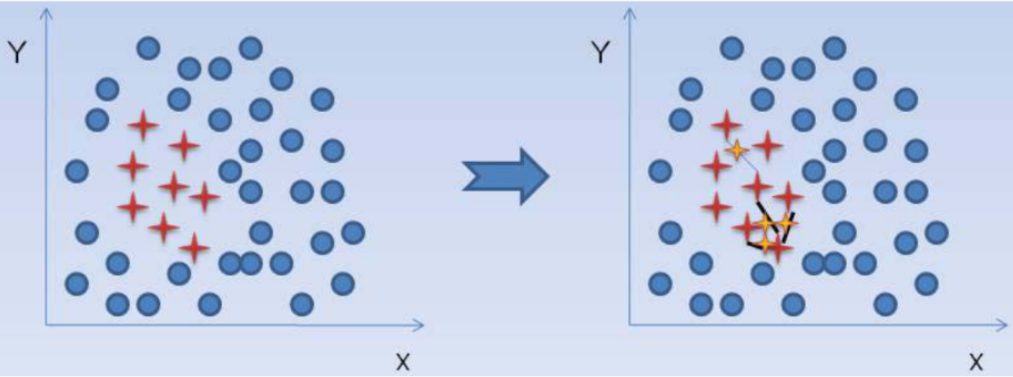
\includegraphics[width=0.7\linewidth]{screenshot008}
	
	\
	
	(b) SMOTE
	
	\
	
	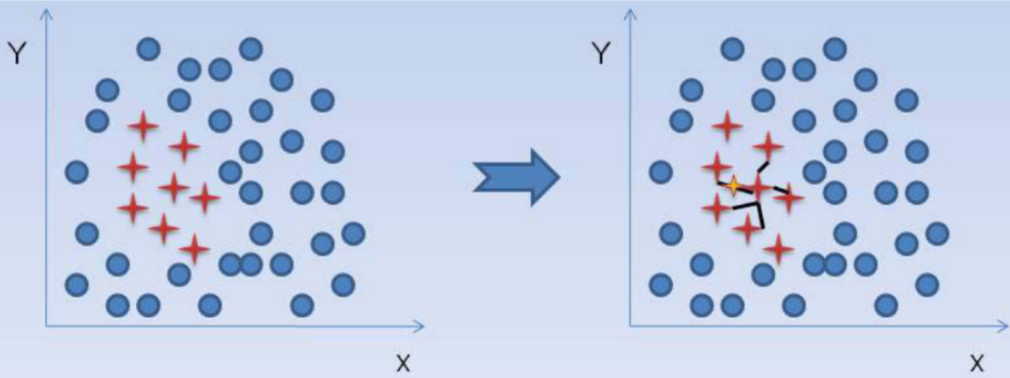
\includegraphics[width=0.7\linewidth]{screenshot009}
	\caption{Отличия  методов синтетической выборки  ADASYN  и  SMOTE. Источник:A Novel Resampling Technique for Imbalanced Dataset Optimization}
		
	
	\label{fig:screenshot008}
\end{figure}



У ADASYN есть два основных недостатка:
\begin{enumerate}
	\item Для редко распределенных миноритарных  классов  может возникнуть ситуация, когда каждая окрестность такого наблюдения будет содержать только 1 наблюдение из   миноритарного  класса.
	\item  Точность метода ADASYN может быть ниже из-за адаптивной природы алгоритма.
\end{enumerate}

Чтобы решить первую проблему, окрестности точек только с 1 наблюдением могут просто дублированное $g_{\mathrm{i}}$  раз, либо такие окрестности можно просто игнорировать при создании синтетических подвыборок, либо можно увеличить размер окрестности.

Вторая проблема возникает из-за того, что больше данных генерируется в районах с большим количеством наблюдений  для мажоритрного класса. Из-за этого сгенерированные синтетические данные могут быть очень похожи на данные мажоритарного  класса, что может привести к большому количеству ложно-положительных результатов. Одним из решений является установление ограничений сверху для $g_{\mathrm{i}}$, для того, чтобы в таких районов не было  сгенерировано слишком много наблюдений.
Вывод

Итак, самым большим преимуществом ADASYN является его адаптивный характер, позволяющий генерировать данные миноритарного класса  для «более сложных для изучения». 


Далее разберем методы 
случайного  удаление примеров мажоритарного класса (Undersampling).  
Во-первых, аналогично методам дублирования, существует наивный способ случайного удаления объектов мажоритарного класса. В частности,  случайным образом наблюдения мажоритарного класса удаляются из набора данных. Это один из простейших методов, используемых для устранения дисбаланса в наборе данных, однако он может увеличить дисперсию классификатора и может с большой вероятностью может  случайно удалить полезные и  важные наблюдения  выборки. 

Во-вторых, популярным алгоритмом является  метод связей Томека (Tomek links). Метод связей Томека позволяет удалить  нежелательные повторяющиеся наблюдения, где связи мажоритарного класса  удаляются до тех пор, пока все минимально удаленные пары ближайших соседей не будут принадлежать к одному и тому же классу. Связь Томека  определяется следующим образом: 
\begin{itemize}
	\item для пары наблюдений  $\operatorname{ir}\left(x_{i}, x_{j}\right)$, где  $x_{i} \in S_{\min }, x_{j} \in S_{\max }$ и $d\left(x_{i}, x_{j}\right)$  — расстояние между $x_{i}$ и  $x_{j}$,  пара  $(x_{i },x_{j})$  называется связанной по  Томеку, если не существует наблюдения  $x_{k}$ такого, что  $d\left(x_{i}, x_{k}\right)<d\left(x_{i}, x_{j}\right)$   или $d\left(x_{j}, x_{k}\right)<d\left(x_{i}, x_{j}\right)$.
\end{itemize}

 Таким образом, если два экземпляра образуют связь  Томека, то либо один из этих наблюдений является шумом, либо оба находятся близко с границей класса, а следовательно такие пары наблюдений, можно использовать для устранения дублирования между классами. Удалив такие дубликаты, можно создать четко определенные кластеры в обучающем наборе и повысить эффективность классификации.


\begin{figure}
	\centering
	
\includegraphics[width=0.7\linewidth]{screenshot011}
   \caption{Принцип работы метода связей Томека. Источник:A Novel Resampling Technique for Imbalanced Dataset Optimization}
	\label{fig:screenshot011}
\end{figure}


Стоит отметить, что существуют  гибридные методы ресэмплинга, объединяющие методы дублирования и случайное удаления объектов выборки. 




\newpage


\nocite{*}  %Чтобы в список литературы напечаталичь все источники из bib-файла

% Если нам хочется, чтобы в списке литературы были не полуторные интервалы можно воспользоваться следующим приёмом: 
\begingroup
\setstretch{1}
\addcontentsline{toc}{chapter}{Список литературы}

\printbibliography[title = Список литературы]

\endgroup





\end{document}
